\documentclass[bac, screen]{bai-thesis}
\usepackage{thesis}

%-------------------------------------------------------------------------------
% Packages and macros
\usepackage{verbatim}
%-------------------------------------------------------------------------------
%Uncomment if you want to use acronyms, and add your acronyms here

%\usepackage[acronym,shortcuts,nonumberlist,nopostdot]{glossaries}
%\makeglossaries
%\newacronym{ros}{ROS}{Robot Operating System}
%\newacronym{vr}{VR}{Virtual Reality}

%-------------------------------------------------------------------------------
% Title information
%-------------------------------------------------------------------------------
\title{Investigating embedding-level parameter-efficient fine-tuning as an alternative to LoRA}

\author{Sailina Singh Chaudhary}
\date{\today}

% Select the subject
\subject{Information Retrieval}

% Academic Year
\AY{2024/2025}

\supervisor{Dr. Gabriella Pasi, University of Milano-Biccoca,}
\supervisor{Marco Braga, University of Milano-Biccoca}
%-------------------------------------------------------------------------------

%-------------------------------------------------------------------------------
\begin{document}
\maketitle
%-------------------------------------------------------------------------------
% \frontmatter
%-------------------------------------------------------------------------------
\chapter*{Abstract}
\addcontentsline{toc}{chapter}{Abstract}
\begin{sloppypar}

Neural re-ranking models based on pre-trained transformers have achieved strong performance in Information Retrieval. In particular, BERT-based cross-encoders such as MonoBERT improve passage ranking by jointly encoding queries and candidate passages. However, full fine-tuning of BERT-large requires updating hundreds of millions of parameters, resulting in high computational, memory, and storage costs.

This thesis investigates embedding-level Parameter-Efficient Fine-Tuning (PEFT), a family of methods that freeze most of a pre-trained model's parameters and update only a small subset, for neural passage re-ranking, and studies whether selected embedding parameters can serve as compact adaptation targets compared with established PEFT methods such as LoRA. The work is motivated by Light-MonoT5, which shows that MonoT5 can be adapted by training only selected prompt-token embeddings while keeping the remaining model parameters frozen. This idea is transferred to a MonoBERT-style cross-encoder by restricting training to selected BERT embeddings, beginning with the structural tokens \texttt{[CLS]} and \texttt{[SEP]}.

The thesis compares this embedding-level approach against a range of alternatives at different parameter budgets, including selected attention-matrix tuning, LoRA applied at different scales, and full MonoBERT fine-tuning, with BM25 and a publicly available MonoBERT checkpoint included as reference baselines. Experiments are conducted using MS MARCO passage ranking data and evaluated on TREC DL 2019, TREC DL 2020, MS MARCO Dev Small, and DL-Hard.

The results show that embedding-level fine-tuning provides extreme parameter efficiency but limited ranking effectiveness compared with attention-based adaptation. LoRA applied to all attention matrices achieves performance close to publicly available MonoBERT and full fine-tuning, while LoRA applied only to the most changed attention matrices provides a strong restricted PEFT approach. Overall, the findings indicate that structural embedding tuning provides insight into model adaptation behaviour, but is not sufficient as a replacement for attention-level adaptation in BERT-based passage re-ranking.
\keywords{Information Retrieval, Passage Re-ranking, BERT, MonoBERT, MonoT5, Parameter-Efficient Fine-Tuning, LoRA, Embedding-Level Adaptation}

\end{sloppypar}
\include{contents}
%-------------------------------------------------------------------------------
\chapter{Introduction}
\label{ch:introduction}

\section{Introduction}
\label{sec:introduction}

Information Retrieval (IR) is the field concerned with retrieving information that satisfies a user's information need from a large collection of documents or passages. Search engines, question answering systems, digital libraries, and many other applications rely on retrieval systems to identify relevant information and present it in an effective order. In this setting, ranking is critical. A system that retrieves a relevant passage but places it too low in the ranking may still fail from the user's perspective, since users typically examine only the highest-ranked results.

For many years, retrieval systems have relied on lexical models such as BM25. These methods remain strong and widely used because they are efficient, scalable, and robust. They estimate relevance using term matching signals, term importance, and document-length normalization. However, lexical retrieval has a fundamental limitation: it relies primarily on surface-level word overlap. A passage can be highly relevant even when it does not contain the exact terms used in the query. For example, a query about ``pregnancy and caffeine'' may be answered by a passage discussing ``coffee consumption during gestation''. Lexical models may struggle in such cases because the semantic relationship between the query and passage is not explicitly represented.

Neural ranking models address this limitation by learning contextual representations from data. Transformer-based language models have become particularly effective for Information Retrieval. BERT, originally introduced for language understanding tasks, can be adapted as a cross-encoder for passage re-ranking \cite{devlin2018bert,nogueira2019passage}. In this setting, the query and candidate passage are jointly encoded:

\begin{equation}
    \texttt{[CLS]} \; q \; \texttt{[SEP]} \; d \; \texttt{[SEP]},
\end{equation}

where $q$ denotes the query and $d$ denotes the candidate passage. This formulation allows query and passage tokens to interact through self-attention. The final representation of the \texttt{[CLS]} token is then used by a classification head to predict passage relevance. When applied to passage ranking, this approach is commonly referred to as MonoBERT.

MonoBERT and other cross-encoder models are effective because they model query-passage interactions directly. However, this effectiveness comes at a high computational cost. Full fine-tuning of BERT-large requires updating hundreds of millions of parameters. This increases memory requirements during training, increases optimizer storage, and produces large task-specific checkpoints. These limitations become increasingly important when adapting models to multiple tasks or domains.

Parameter-Efficient Fine-Tuning (PEFT) methods aim to reduce this cost by freezing most of the pre-trained model and updating only a smaller subset of parameters. LoRA is one of the most widely adopted PEFT approaches \cite{hu2021lora}. Instead of modifying the original model weights directly, LoRA introduces trainable low-rank updates while keeping the original parameters frozen. It has shown strong adaptation performance while requiring substantially fewer trainable parameters than full fine-tuning.

This thesis investigates a more restrictive form of parameter-efficient adaptation: embedding-level fine-tuning. Instead of introducing additional parameters or modifying internal transformer weights, it studies whether selected token embeddings can serve as compact adaptation targets for BERT-based passage re-ranking. This idea is motivated by Light-MonoT5, which investigates whether MonoT5 can be adapted by training only selected prompt-token embeddings while keeping the remaining model parameters frozen \cite{braga2025monot5}. This suggests that some task-specific adaptation behaviour may be captured by a small subset of parameters.

The central idea of this thesis is to transfer this principle from MonoT5 to MonoBERT. However, the transfer is not direct because the two architectures use different mechanisms for relevance prediction. MonoT5 is a sequence-to-sequence model that predicts relevance through generated tokens, whereas MonoBERT is an encoder-only cross-encoder that predicts relevance through a classification head. Therefore, the adaptation targets must be reconsidered. In BERT, the input structure is defined by special tokens, particularly \texttt{[CLS]} and \texttt{[SEP]}. The \texttt{[CLS]} token provides the representation used by the classifier, while \texttt{[SEP]} separates the query and passage segments.

This leads to the main research question of this thesis: can a BERT cross-encoder be adapted for passage re-ranking by training only selected embeddings, particularly the embeddings of structural tokens such as \texttt{[CLS]} and \texttt{[SEP]}? If successful, such an approach would provide an extremely parameter-efficient adaptation mechanism. In BERT-large, each embedding vector has dimension 1024, meaning that training only these two token embeddings updates only 2048 parameters.

The objective of this thesis is not to assume that embedding-only adaptation can replace full fine-tuning. Instead, embedding-level tuning is investigated as a controlled experiment to understand where task-specific adaptation occurs in MonoBERT. If selected embeddings provide strong performance, this would indicate that a small number of input-level parameters contain substantial adaptation information. If performance is limited, this would suggest that deeper model components are required. To investigate this, embedding-level approaches are compared with selected attention-matrix tuning, LoRA-based adaptation, publicly available MonoBERT, BM25, and full MonoBERT fine-tuning.

\section{Problem Formulation}
\label{sec:introduction_problem}

The task investigated in this thesis is passage re-ranking. Given a query $q$ and an initial candidate set of passages:

\begin{equation}
    C_q = \{d_1, d_2, \ldots, d_k\},
\end{equation}

the objective is to learn a scoring function:

\begin{equation}
    s(q,d_i) \rightarrow \mathbb{R},
\end{equation}

that estimates the relevance of each candidate passage $d_i$ with respect to the query. The final ranking is obtained by sorting the candidate passages according to their predicted relevance scores.

The models studied in this thesis operate as second-stage re-rankers. They do not retrieve passages directly from the complete document collection. Instead, an initial retrieval system first produces a candidate set, and the neural re-ranker attempts to improve the ordering of these candidates. This setting is particularly suitable for cross-encoder models because they provide strong query-passage interaction modelling, but require separate inference for each query-passage pair.

The standard approach for adapting BERT-based re-rankers is full fine-tuning, where all model parameters are updated:

\begin{equation}
    \theta^\ast = \arg\min_{\theta} \mathcal{L}_{task}(\theta).
    \label{eq:full_finetune_objective}
\end{equation}

Although effective, full fine-tuning requires updating and storing the complete model. Parameter-Efficient Fine-Tuning instead keeps the original parameters frozen and optimizes only a smaller set of task-specific parameters:

\begin{equation}
    \phi^\ast = \arg\min_{\phi} \mathcal{L}_{task}(\theta_0,\phi).
    \label{eq:peft_objective}
\end{equation}

where $\theta_0$ represents the frozen pre-trained model parameters and $\phi$ represents the trainable adaptation parameters.

The central question of this thesis is how small and restricted the trainable parameter set can be while still producing effective passage re-ranking performance. Different forms of $\phi$ are therefore investigated, including selected embedding vectors, selected attention matrices, LoRA adapters, and full model parameters.

The thesis is guided by the following research questions:

\begin{itemize}

    \item \textbf{RQ1:} Can a BERT cross-encoder be adapted for passage re-ranking by training only selected embedding vectors?

    \item \textbf{RQ2:} How does training only the structural token embeddings \texttt{[CLS]} and \texttt{[SEP]} compare with training the embedding rows that change most between BERT and MonoBERT?

    \item \textbf{RQ3:} Are the strongest task-specific changes between BERT and MonoBERT concentrated more strongly in embedding parameters or attention parameters?

    \item \textbf{RQ4:} How does embedding-level adaptation compare with LoRA-based parameter-efficient fine-tuning?

    \item \textbf{RQ5:} Can LoRA applied only to the most changed attention matrices retain a substantial proportion of the performance achieved by applying LoRA to all attention matrices?

    \item \textbf{RQ6:} Does locally fine-tuned MonoBERT achieve results comparable to a publicly available MonoBERT checkpoint, validating the experimental pipeline?

\end{itemize}

To answer these questions, the thesis evaluates a sequence of controlled experiments. The first experiment trains only the embeddings of \texttt{[CLS]} and \texttt{[SEP]}. Additional experiments train the most changed embedding rows, the most changed attention matrices, the complete embedding layer, and all embeddings except the structural tokens. LoRA is evaluated both across all attention matrices and only on selected attention matrices. BM25, publicly available MonoBERT, and full MonoBERT fine-tuning are included as reference systems.

\section{Outline}
\label{sec:introduction_outline}

The remainder of this thesis is organized as follows.

\vspace{\baselineskip}

\textbf{Chapter~\ref{ch:background}} introduces the background required for this research. It covers classical Information Retrieval, BM25, evaluation metrics, transformer architectures, BERT, MonoBERT, MonoT5, LoRA, task arithmetic, and embedding-level adaptation.

\vspace{\baselineskip}

\textbf{Chapter~\ref{ch:methodology}} presents the proposed methodology. It describes how the Light-MonoT5 prompt-embedding idea is transferred to BERT, how BERT and MonoBERT parameters are compared, how embedding-level gradient masking is implemented, and how the different adaptation strategies are defined.

\vspace{\baselineskip}

\textbf{Chapter~\ref{ch:experiments}} describes the experimental setup. It presents the implementation environment, training data, evaluation datasets, candidate generation procedure, training configuration, checkpointing strategy, and verification procedures used during experimentation.

\vspace{\baselineskip}

\textbf{Chapter~\ref{ch:results}} presents the experimental results and analysis. It compares embedding-level adaptation, attention-matrix tuning, LoRA-based approaches, publicly available MonoBERT, full MonoBERT fine-tuning, and BM25 across the evaluated datasets.

\vspace{\baselineskip}

\textbf{Chapter~\ref{ch:conclusions}} summarizes the main findings of the thesis, answers the research questions, discusses limitations, and presents possible directions for future research.
\chapter{Background and Related Work}
\label{ch:background}

This chapter introduces the background required for this thesis. The work is positioned at the intersection of Information Retrieval, neural passage re-ranking, and parameter-efficient fine-tuning. The chapter first introduces the retrieval problem and classical lexical ranking methods. It then presents evaluation metrics, neural re-ranking, transformers, BERT, MonoBERT, and MonoT5. Finally, it discusses parameter-efficient fine-tuning methods, with particular attention to LoRA, task arithmetic in Information Retrieval, and embedding-level adaptation.

\section{Information Retrieval}
\label{sec:background_ir}

Information Retrieval (IR) studies methods for finding and ranking information items that satisfy a user's information need within a collection \cite{manning2008ir}. The user expresses an information need through a query, and the retrieval system returns a ranked list of documents or passages. A document is useful only if it is relevant and ranked sufficiently high to be observed by the user.

Formally, given a collection:

\begin{equation}
    \mathcal{D} = \{d_1, d_2, \ldots, d_N\},
\end{equation}

and a query $q$, a retrieval system assigns a relevance score:

\begin{equation}
    s(q,d_i) \rightarrow \mathbb{R}.
\end{equation}

The documents are then ordered according to their scores. The objective of the scoring function is to estimate the relevance of each document to the query.

A central challenge in IR is that relevance is not directly observable. Queries are often short descriptions of a user's information need, and relevance judgments may vary between users. Retrieval systems therefore approximate relevance using lexical matching, learned representations, user behaviour signals, or supervised relevance annotations.

\subsection{Ranking and the Probability Ranking Principle}
\label{subsec:background_prp}

The Probability Ranking Principle provides a theoretical foundation for ranked retrieval. Under its assumptions, documents should be ranked in decreasing order of their probability of relevance \cite{manning2008ir}. If $R$ is a binary relevance variable, the ideal ranking orders documents according to:

\begin{equation}
    P(R=1 \mid q,d).
\end{equation}

In practice, this probability is unknown. Retrieval models therefore compute scores that approximate relevance. Classical retrieval models estimate relevance using term statistics, while neural retrieval models learn relevance patterns from data.

\subsection{Passage Retrieval}
\label{subsec:background_passage}

This thesis focuses on passage retrieval and passage re-ranking. In passage retrieval, the retrieval unit is a short text passage rather than an entire document. This setting is common in question answering and web search, where a user's information need may be satisfied by a concise text segment.

Passage retrieval differs from document retrieval because passages are shorter and typically contain more focused information. However, the number of retrievable units increases significantly, creating additional challenges for retrieval systems. The MS MARCO passage ranking dataset used in this thesis contains millions of passages and real user queries \cite{nguyen2016msmarco}.

\subsection{Two-Stage Retrieval Pipelines}
\label{subsec:background_two_stage}

Modern neural retrieval systems commonly use a two-stage architecture \cite{lin2021pretrained}. The first stage retrieves an initial candidate set from the full collection. Since this stage must search millions of documents or passages, efficiency is the primary requirement. Lexical retrieval models such as BM25 and dense retrieval models are commonly used for this purpose.

The second stage re-ranks the candidate set using a more accurate but computationally expensive model. Cross-encoders are particularly suitable for this stage because they jointly encode the query and passage, allowing detailed token-level interaction.

This thesis studies second-stage passage re-ranking. The neural models are not responsible for retrieving passages from the complete collection. Instead, they receive candidate passages and reorder them according to predicted relevance.

\section{Classical Lexical Retrieval}
\label{sec:background_lexical}

Classical retrieval models rely on lexical matching between queries and documents. They assume that relevant documents often contain terms that are important to the user's query. Although neural retrieval methods provide stronger semantic modelling capabilities, lexical retrieval remains an important baseline due to its efficiency and effectiveness.

\paragraph{Term Frequency and Inverse Document Frequency}
\label{subsec:background_tfidf}

A fundamental concept in lexical retrieval is that terms should be weighted according to their discriminative value. A term appearing frequently in a document may indicate importance, but a term appearing in almost every document provides little information. This motivates the use of term frequency and inverse document frequency.

The inverse document frequency of a term $t$ is commonly defined as:

\begin{equation}
    \operatorname{idf}(t) =
    \log \frac{N}{df_t},
\end{equation}

where $N$ is the number of documents in the collection and $df_t$ is the number of documents containing the term. Rare terms receive higher weights because they provide stronger discrimination between relevant and non-relevant documents.

\paragraph{BM25}
\label{subsec:background_bm25}

BM25 is one of the most widely used lexical ranking functions \cite{robertson2009probabilistic}. It is based on probabilistic retrieval and improves over basic TF-IDF by incorporating term-frequency saturation and document-length normalization.

A common formulation of BM25 is:

\begin{equation}
    \operatorname{BM25}(q,d)
    =
    \sum_{t \in q}
    \operatorname{idf}(t)
    \frac{f(t,d)(k_1+1)}
    {f(t,d)+k_1\left(1-b+b\frac{|d|}{\operatorname{avgdl}}\right)},
\end{equation}

where $f(t,d)$ represents the frequency of term $t$ in document $d$, $|d|$ is document length, $\operatorname{avgdl}$ is the average document length, and $k_1$ and $b$ are hyperparameters.

BM25 remains important for two reasons. First, it is computationally efficient and can scale to large collections. Second, it provides a strong baseline that neural retrieval methods must improve upon. In this thesis, BM25 is used both as a retrieval baseline and as the candidate generator for the DL-Hard evaluation setting.

\section{Evaluation Metrics in Information Retrieval}
\label{sec:background_metrics}

Evaluation in IR is performed by comparing ranked results against relevance judgments. Since users typically examine only the highest-ranked results, many evaluation metrics emphasize ranking quality near the top of the list.

\paragraph{nDCG@10}
\label{subsec:background_nDCG}

Normalized Discounted Cumulative Gain is commonly used when relevance judgments contain multiple levels of relevance. Discounted Cumulative Gain at rank $k$ is defined as:

\begin{equation}
    \operatorname{DCG@}k =
    \sum_{i=1}^{k}
    \frac{2^{rel_i}-1}{\log_2(i+1)},
\end{equation}

where $rel_i$ represents the relevance grade of the document at rank $i$. The logarithmic discount reduces the contribution of relevant documents appearing lower in the ranking.

nDCG normalizes DCG by the ideal ranking:

\begin{equation}
    \operatorname{nDCG@}k =
    \frac{\operatorname{DCG@}k}{\operatorname{IDCG@}k}.
\end{equation}

This thesis reports nDCG@10 because it measures the quality of the highest-ranked results, which are most important in practical search systems.

\paragraph{MRR@10}
\label{subsec:background_mrr}

Mean Reciprocal Rank measures how early the first relevant result appears in a ranked list. For an individual query, reciprocal rank is defined as:

\begin{equation}
    \operatorname{RR} = \frac{1}{r},
\end{equation}

where $r$ is the rank position of the first relevant passage. MRR@10 averages reciprocal rank over all queries while considering only the top ten ranking positions. If no relevant passage appears within the first ten positions, the query receives a score of zero.

MRR is particularly useful for tasks where finding a single relevant result near the top of the ranking is important, making it a common metric for MS MARCO-style passage ranking.

\paragraph{MAP@1000}
\label{subsec:background_map}

Mean Average Precision evaluates how effectively a system ranks all relevant documents across queries. For a query with relevant set $R$, Average Precision at rank $k$ is:

\begin{equation}
    \operatorname{AP@}k =
    \frac{1}{|R|}
    \sum_{i=1}^{k}
    P@i \cdot \mathbb{I}(d_i \in R),
\end{equation}

where $P@i$ represents precision at rank $i$ and $\mathbb{I}$ is an indicator function. MAP@1000 averages AP@1000 over all queries.

\paragraph{Recall@100}
\label{subsec:background_recall}

Recall@100 measures the fraction of relevant passages that appear within the first 100 ranked positions:

\begin{equation}
    \operatorname{Recall@}100 =
    \frac{|R \cap D_{100}|}{|R|}.
\end{equation}

In a re-ranking setting, Recall@100 provides information about whether relevant passages are moved into the upper part of the ranking, even if they are not placed within the top ten positions.

\section{Neural Information Retrieval}
\label{sec:background_neural_ir}

Neural Information Retrieval uses neural models to estimate relevance from learned representations. Unlike purely lexical methods, neural models can capture semantic relationships and contextual information, allowing them to identify relevant passages even when query and passage terms do not exactly overlap.

\subsection{Bi-Encoders}
\label{subsec:background_biencoders}

Bi-encoders independently encode queries and passages:

\begin{equation}
    h_q = f_\theta(q), \qquad h_d = g_\theta(d).
\end{equation}

The resulting representations are compared using a similarity function:

\begin{equation}
    s(q,d) = \operatorname{sim}(h_q,h_d).
\end{equation}

Bi-encoders are computationally efficient because document representations can be precomputed and stored in an index. However, the query and passage interact only through the final similarity calculation, limiting fine-grained token-level interaction.

\subsection{Cross-Encoders}
\label{subsec:background_crossencoders}

Cross-encoders jointly encode the query and passage as a single input sequence. This allows direct interaction between query and passage tokens throughout the model. The resulting representation is then used to estimate relevance.

The advantage of cross-encoders is their ability to model detailed interactions between query and passage terms. However, they are computationally expensive because every query-passage pair requires an independent forward pass.

For this reason, cross-encoders are primarily used for second-stage re-ranking rather than first-stage retrieval. This thesis focuses on BERT-based cross-encoder re-ranking.

\section{Transformers}
\label{sec:background_transformers}

Transformers are neural architectures based on self-attention, which allows every token representation to attend to all other tokens in the sequence \cite{vaswani2017attention}. Given an input representation matrix $X$, attention computes query, key, and value projections:

\begin{equation}
    Q=XW_Q, \qquad K=XW_K, \qquad V=XW_V.
\end{equation}

The attention output is:

\begin{equation}
    \operatorname{Attention}(Q,K,V)
    =
    \operatorname{softmax}
    \left(
    \frac{QK^\top}{\sqrt{d_k}}
    \right)V.
\end{equation}

Multi-head attention performs this operation using multiple projection matrices, allowing the model to capture different types of relationships between tokens.

Self-attention is particularly important for passage re-ranking because relevance often depends on interactions between query and passage terms. Encoder-only transformer models such as BERT use stacked self-attention layers to produce contextualized token representations.

\section{BERT}
\label{sec:background_bert}

BERT is an encoder-only transformer model pre-trained using self-supervised objectives, most notably masked language modelling \cite{devlin2018bert}. Unlike autoregressive language models, BERT uses bidirectional context, allowing each token representation to depend on surrounding tokens.

For sentence-pair tasks, BERT uses special tokens and segment information. The \texttt{[CLS]} token is placed at the beginning of the sequence and provides a representation used for classification. The \texttt{[SEP]} token separates different text segments.

For passage re-ranking, the input format is:

\begin{equation}
    \texttt{[CLS]} \; q \; \texttt{[SEP]} \; d \; \texttt{[SEP]}.
\end{equation}

The final hidden representation of \texttt{[CLS]} is passed to a classification layer. The model produces logits corresponding to relevant and non-relevant classes. During standard fine-tuning, both the encoder and classification head are updated, while PEFT methods restrict which parameters are trainable.

\section{MonoBERT}
\label{sec:background_monobert}

MonoBERT applies BERT to passage re-ranking by treating every query-passage pair as an independent classification problem \cite{nogueira2019passage}. The model estimates the probability that a passage is relevant to a query, and candidate passages are sorted according to their predicted relevance scores.

MonoBERT achieves strong ranking effectiveness because it uses the full contextual modelling capability of BERT for each query-passage pair. However, this also introduces significant computational cost. For example, re-ranking 1000 candidate passages requires 1000 separate model evaluations.

This computational cost makes MonoBERT unsuitable for first-stage retrieval over very large collections, but practical for second-stage re-ranking. In the original MonoBERT setting, the complete BERT model is fine-tuned on passage ranking data. In this thesis, MonoBERT serves both as a reference model and as the target setting for investigating embedding-level adaptation.

\section{MonoT5 and Light-MonoT5}
\label{sec:background_monot5}

MonoT5 reformulates document ranking as a sequence-to-sequence generation problem \cite{nogueira2020document}. Instead of directly predicting a relevance score, the model receives a query-document pair and generates a relevance token such as ``true'' or ``false''. The probability assigned to the relevant token is then used as the ranking score.

Light-MonoT5 investigates the adaptation behaviour of MonoT5 and studies whether effective ranking performance can be achieved by training only selected prompt-token embeddings \cite{braga2025monot5}. The method is motivated by the observation that a small subset of parameters may contain useful task-specific adaptation information.

The adaptation principle explored in Light-MonoT5 motivates this thesis. However, the two settings are not identical. MonoT5 uses a sequence-to-sequence architecture with explicit textual prompts, whereas MonoBERT is an encoder-only cross-encoder without prompt generation. Therefore, this thesis adapts the idea of selective embedding training to the BERT input structure by investigating structural tokens such as \texttt{[CLS]} and \texttt{[SEP]}.

\section{Parameter-Efficient Fine-Tuning}
\label{sec:background_peft}

As introduced in Section~\ref{sec:introduction_problem}, full fine-tuning updates all parameters of a pre-trained model (Equation~\ref{eq:full_finetune_objective}), whereas Parameter-Efficient Fine-Tuning (PEFT) instead freezes most model parameters and optimizes only a small set of additional or selected parameters, $\phi$ (Equation~\ref{eq:peft_objective}), where $\theta_0$ represents frozen base-model parameters.

PEFT methods reduce memory usage, training cost, and checkpoint size. They also enable multiple task-specific adaptations to share the same frozen base model.

\section{LoRA}
\label{sec:background_lora}

Low-Rank Adaptation (LoRA) is one of the most widely used PEFT methods \cite{hu2021lora}. LoRA freezes a pre-trained weight matrix $W_0$ and learns a low-rank update:

\begin{equation}
    W = W_0 + \Delta W,
\end{equation}

where:

\begin{equation}
    \Delta W = BA.
\end{equation}

The matrices $A$ and $B$ are trainable low-rank matrices whose rank $r$ is much smaller than the dimensions of the original weight matrix. This significantly reduces the number of trainable parameters.

LoRA is commonly applied to attention projection matrices because these matrices contain important task-related transformations in transformer models. In this thesis, LoRA is used as the primary PEFT baseline and is compared against embedding-level and directly trained attention-level adaptation methods.


\section{Task Arithmetic for Information Retrieval}
\label{sec:background_task_arithmetic}

Task arithmetic studies model adaptation by analysing differences between model parameters. In Information Retrieval, task vectors have been used to represent adaptation as the parameter difference between a pre-trained model and a task-adapted model \cite{braga2025taskarithmetic}.

This perspective motivates the parameter-change analysis used in this thesis. If the difference between BERT and MonoBERT identifies parameters that change strongly during IR adaptation, these parameters may represent useful adaptation targets. This motivates experiments that train the most changed embedding rows and the most changed attention matrices.

\section{Embedding-Level Adaptation}
\label{sec:background_embedding_adaptation}

Embedding-level adaptation restricts training to selected rows of the embedding matrix. Let:

\begin{equation}
    E \in \mathbb{R}^{|V| \times h}
\end{equation}

represent the word embedding matrix, where $|V|$ is the vocabulary size and $h$ is the hidden dimension. Each token ID corresponds to one row of this matrix.

If $S$ represents the set of trainable token IDs, only rows belonging to $S$ receive updates:

\begin{equation}
    \Delta E_i' =
    \begin{cases}
    \Delta E_i & \text{if } i \in S,\\
    0 & \text{otherwise}.
    \end{cases}
\end{equation}

The masked update $\Delta E'$ is applied during optimization, ensuring that all non-selected embeddings remain unchanged.

In BERT-large, each embedding vector has dimension 1024. Therefore, training only the \texttt{[CLS]} and \texttt{[SEP]} embeddings updates only:

\begin{equation}
    2 \times 1024 = 2048
\end{equation}

parameters. This makes the approach extremely parameter-efficient, but also highly restrictive.

Embedding-level adaptation can be interpreted as a form of input-structure tuning. It modifies how selected tokens enter the frozen transformer, but it does not directly change internal transformer computations. Whether this limited adaptation capacity is sufficient for passage re-ranking is the central empirical question investigated in this thesis.


\section{Summary}
\label{sec:background_summary}

This chapter introduced the concepts required to understand the thesis. Classical Information Retrieval provides the retrieval formulation, BM25 baseline, and evaluation metrics. Neural Information Retrieval introduces cross-encoders such as MonoBERT, which provide strong ranking effectiveness but require substantial computation. MonoT5 and Light-MonoT5 motivate the idea that selected embeddings may serve as compact adaptation points. PEFT methods such as LoRA reduce adaptation cost by training only a subset of parameters. Task arithmetic further supports the broader idea that adaptation can be studied through parameter selection.

The next chapter describes how these ideas are translated into the methodology used to investigate embedding-level adaptation for BERT-based passage re-ranking.
\chapter{Methodology}
\label{ch:methodology}

This chapter describes the methodology used to investigate embedding-level parameter-efficient fine-tuning for BERT-based passage re-ranking. The objective is to evaluate whether selected embeddings can serve as compact adaptation points for MonoBERT-style Information Retrieval, and to compare this strategy against attention-level adaptation, LoRA, and full fine-tuning.

The methodology follows the motivation of the thesis. First, the Light-MonoT5 prompt-embedding idea is transferred to the BERT cross-encoder setting. Second, a BERT-to-MonoBERT parameter-change analysis is used to identify which embeddings and internal matrices exhibit the largest changes during IR adaptation. Third, controlled training approaches are defined, ranging from extremely small embedding-level updates to full model fine-tuning.

\section{Task Definition}
\label{sec:methodology_task}

The task considered in this thesis is passage re-ranking. Given a query $q$, an initial retrieval stage provides a set of candidate passages:

\begin{equation}
    C_q = \{d_1,d_2,\ldots,d_k\}.
\end{equation}

The re-ranker assigns a relevance score to each query-passage pair:

\begin{equation}
    s_i = f_\theta(q,d_i),
\end{equation}

and the candidate set is sorted according to decreasing score:

\begin{equation}
    \pi_q = \operatorname{rank}_{d_i \in C_q} s_i.
\end{equation}

The models investigated in this thesis are not first-stage retrieval systems. They do not retrieve documents from the complete corpus. Instead, they operate on an existing candidate set and attempt to improve the ranking order. This setting matches the typical use case of cross-encoder re-rankers, which provide stronger relevance estimation at a higher computational cost.

\section{Base Model}
\label{sec:methodology_base_model}

The base neural architecture is \texttt{bert-large-uncased}, used as a sequence classification cross-encoder. BERT-large contains 24 Transformer encoder layers, a hidden dimension of 1024, and 16 attention heads. The complete model contains approximately 335 million parameters.

For passage re-ranking, the query and passage are concatenated into a single BERT input sequence:

\begin{equation}
    x = \texttt{[CLS]} \oplus q \oplus \texttt{[SEP]} \oplus d \oplus \texttt{[SEP]}.
\end{equation}

The final contextual representation of the \texttt{[CLS]} token is passed to a classification head. The model outputs two logits corresponding to non-relevant and relevant classes. During evaluation, the relevance-class logit is used as the ranking score.

This architecture follows the MonoBERT passage re-ranking formulation \cite{nogueira2019passage}. Since the final prediction depends on the contextual representation of \texttt{[CLS]}, and query-passage interaction occurs throughout the Transformer layers, it provides a suitable setting for studying where task-specific adaptation occurs.

\section{From Light-MonoT5 to MonoBERT}
\label{sec:methodology_light_monot5_transfer}

The initial motivation of this thesis comes from Light-MonoT5, which investigates whether a MonoT5 model can be adapted by updating only selected prompt-token embeddings while keeping the remaining parameters frozen \cite{braga2025monot5}. The key idea is that a small subset of parameters may contain sufficient capacity for task adaptation.

This thesis investigates whether a similar principle can be transferred to BERT-based passage re-ranking. However, MonoT5 and MonoBERT differ architecturally. MonoT5 is a sequence-to-sequence model where prompt tokens influence the generated output sequence, whereas MonoBERT is a cross-encoder where relevance is predicted from the final contextual representation of the input sequence.

Therefore, the closest BERT equivalent to prompt-token adaptation is to update embeddings associated with structural tokens that appear in every query-passage input. The two selected tokens are:

\begin{itemize}
    \item \texttt{[CLS]}, whose contextual representation is used by the classification head;
    \item \texttt{[SEP]}, which separates the query and passage segments.
\end{itemize}

The first proposed experiment therefore trains only the embeddings of \texttt{[CLS]} and \texttt{[SEP]}. This provides a direct test of whether a highly restricted embedding-level update can adapt a frozen MonoBERT-style model.

\section{Training Data Construction}
\label{sec:methodology_training_data}

All trainable neural approaches are trained using MS MARCO passage ranking triples. Each training example contains a query $q$, a relevant passage $d^+$, and a non-relevant passage $d^-$. The triples are converted into binary classification examples:

\begin{align}
    (q,d^+) &\rightarrow 1, \\
    (q,d^-) &\rightarrow 0.
\end{align}

The model is optimized using cross-entropy loss over the two relevance classes. Each example follows the standard MonoBERT input format:

\begin{equation}
    \texttt{[CLS]} \; q \; \texttt{[SEP]} \; d \; \texttt{[SEP]}.
\end{equation}

The maximum sequence length is set to 128 tokens. When truncation is required, it is applied to the passage side while preserving the query tokens whenever possible.

\section{Parameter-Change Analysis}
\label{sec:methodology_parameter_change}

Before defining the restricted adaptation approaches, a parameter-change analysis is performed between a pre-trained BERT model and a MonoBERT-style fine-tuned model. The goal is to identify which parts of the model undergo the largest changes during adaptation to passage re-ranking.

This analysis is motivated by the observation that parameter differences between a general model and a task-adapted model may reveal useful adaptation targets. The resulting parameter differences are used to select embedding rows and attention matrices for additional experiments.

For a matrix-valued parameter $W$, the parameter difference is defined as:

\begin{equation}
    \Delta W = W_{\text{MonoBERT}} - W_{\text{BERT}}.
\end{equation}

The Frobenius norm is used to measure the overall magnitude of change:

\begin{equation}
    \|\Delta W\|_F =
    \sqrt{
    \sum_i \sum_j (\Delta W_{ij})^2
    }.
\end{equation}

Since the Frobenius norm is influenced by matrix size, the maximum absolute change is also considered:

\begin{equation}
    \|\Delta W\|_{\max}
    =
    \max_{i,j} |\Delta W_{ij}|.
\end{equation}

For embedding parameters, the analysis is performed at the token level. Given an embedding vector before and after fine-tuning:

\begin{equation}
    e_i^{(0)}, e_i^{(1)},
\end{equation}

the Euclidean distance is calculated as:

\begin{equation}
    d_i =
    \|e_i^{(1)}-e_i^{(0)}\|_2.
\end{equation}

Cosine similarity is additionally measured to compare changes in embedding direction:

\begin{equation}
    \operatorname{cos}(e_i^{(0)},e_i^{(1)})
    =
    \frac{
    e_i^{(0)} \cdot e_i^{(1)}
    }{
    \|e_i^{(0)}\|_2
    \|e_i^{(1)}\|_2
    }.
\end{equation}

The results of this analysis, including the specific embedding rows and attention matrices identified as adaptation targets, are presented in Section~\ref{sec:results_parameter_change} alongside the other experimental results.


\section{Embedding-Level Gradient Masking}
\label{sec:methodology_gradient_masking}

Embedding-level approaches are implemented using gradient masking. Let:

\begin{equation}
    E \in \mathbb{R}^{|V| \times h}
\end{equation}

represent the BERT embedding matrix, where $|V|$ is the vocabulary size and $h=1024$ is the hidden dimension.

A binary mask $M$ with the same dimensions as $E$ is created. Rows corresponding to selected token IDs are assigned a value of 1, while all other rows are assigned 0. During optimization, the embedding gradient is modified as:

\begin{equation}
    G' = G \odot M,
\end{equation}

where $G$ is the original gradient and $\odot$ represents element-wise multiplication.

This ensures that only selected embedding rows receive updates. All remaining parameters are frozen. After training, the embedding matrix is compared with the initial matrix to verify that only the intended rows changed.

For example, in the \texttt{[CLS]}/\texttt{[SEP]} experiment, only token IDs 101 and 102 should be modified. In the all-embeddings-except-\texttt{[CLS]}/\texttt{[SEP]} experiment, these rows should remain unchanged.

\section{Compared Approaches}
\label{sec:methodology_compared_approaches}

The thesis evaluates ten approaches. These approaches are designed to compare different adaptation locations and parameter budgets.

\subsection{BM25}
\label{subsec:methodology_bm25}

BM25 is used as the lexical retrieval baseline. It does not perform neural re-ranking. For DL-Hard, BM25 is additionally used to generate the top-1000 candidate passages that are subsequently re-ranked by neural models.

\subsection{Public MonoBERT}
\label{subsec:methodology_public_monobert}

A publicly available MonoBERT checkpoint is evaluated using the same candidate sets and evaluation pipeline as the other neural models. This provides a reference point for comparing the locally trained models and restricted adaptation methods.

\subsection{CLS/SEP Embedding Tuning}
\label{subsec:methodology_cls_sep}

The first embedding-level experiment updates only the embeddings of \texttt{[CLS]} and \texttt{[SEP]}. For \texttt{bert-large-uncased}, these token IDs are:

\begin{itemize}
    \item \texttt{[CLS]}: 101;
    \item \texttt{[SEP]}: 102.
\end{itemize}

Since each embedding vector has dimension 1024, the number of trainable parameters is:

\begin{equation}
    2 \times 1024 = 2048.
\end{equation}

All other model parameters remain frozen.

\subsection{Top-6 Embedding Tuning}
\label{subsec:methodology_top6}

This approach updates the six vocabulary embedding rows with the largest measured changes between BERT and MonoBERT, identified in Section~\ref{sec:results_parameter_change}:

\begin{equation}
    \{1000, 2133, 29649, 29658, 29645, 21932\}.
\end{equation}

The maximum number of trainable parameters is:

\begin{equation}
    6 \times 1024 = 6144.
\end{equation}

This experiment evaluates whether the largest embedding changes contain useful adaptation information.

\subsection{Top-3 Attention Matrix Tuning}
\label{subsec:methodology_top3_attention}

This approach directly trains the three attention matrices identified by the parameter-change analysis, presented in Section~\ref{sec:results_parameter_change}:

\begin{itemize}
    \item \texttt{bert.encoder.layer.23.attention.output.dense.weight};
    \item \texttt{bert.encoder.layer.22.attention.output.dense.weight};
    \item \texttt{bert.encoder.layer.23.attention.self.query.weight}.
\end{itemize}

Each matrix has dimensions $1024 \times 1024$, resulting in:

\begin{equation}
    3 \times 1024 \times 1024
    =
    3,145,728
\end{equation}

trainable parameters.

Although larger than embedding-only methods, this represents less than 1\% of the complete BERT-large parameter count.

\subsection{All Embeddings}
\label{subsec:methodology_all_embeddings}

This experiment trains the complete word embedding matrix while keeping the Transformer layers and classification head frozen. It evaluates whether embedding-level adaptation becomes effective when the complete input representation space is allowed to change.

\subsection{All Embeddings Except CLS/SEP}
\label{subsec:methodology_all_except_cls_sep}

This experiment trains all vocabulary embeddings except the structural tokens:

\begin{equation}
    S =
    \{1,\ldots,|V|\}
    \setminus
    \{101,102\}.
\end{equation}

The purpose is to compare general vocabulary embedding adaptation against structural-token adaptation.

\subsection{LoRA on All Attention Matrices}
\label{subsec:methodology_lora_all}

LoRA is applied to all attention projection matrices. For a frozen weight matrix $W_0$, LoRA defines the adapted matrix as:

\begin{equation}
    W = W_0 + BA,
\end{equation}

where $A$ and $B$ are trainable low-rank matrices.

The LoRA configuration uses rank 8, scaling factor 16, and dropout 0.05. The total number of trainable parameters is 1,572,864.

\subsection{LoRA on the Top-3 Attention Matrices}
\label{subsec:methodology_lora_top3}

This approach applies LoRA adapters only to the three attention matrices selected through the parameter-change analysis. With rank 8, this results in 49,152 trainable parameters.

This experiment evaluates whether parameter-change analysis can guide adapter placement and reduce the number of trainable parameters while maintaining ranking effectiveness.

\section{Full MonoBERT}
\label{subsec:methodology_full_monobert}

Full MonoBERT fine-tuning updates all parameters of \texttt{bert-large-uncased}. This experiment provides an upper-bound reference for adaptation effectiveness and verifies that the local training and evaluation pipeline produces results comparable to a standard MonoBERT-style model.

\section{Training Configuration}
\label{sec:methodology_training_configuration}

The main training configuration is shown in Table~\ref{tab:methodology_training_config}.

\begin{table}[ht]
\centering
\begin{tabular}{ll}
\hline
\textbf{Setting} & \textbf{Value} \\
\hline
Base model & \texttt{bert-large-uncased} \\
Training data & \texttt{msmarco-passage/train/triples-small} \\
Training steps & 100,000 \\
Maximum sequence length & 128 \\
Effective batch size & 128 \\
Warmup steps & 10,000 \\
Optimizer & AdamW \\
Precision & Mixed precision \\
Checkpoint interval & 10,000 steps \\
\hline
\end{tabular}
\caption{Main training configuration used for the experiments.}
\label{tab:methodology_training_config}
\end{table}

Most parameter-efficient experiments use a micro-batch size of 16 with gradient accumulation over 8 steps, resulting in an effective batch size of 128. Full MonoBERT fine-tuning uses a micro-batch size of 8 with gradient accumulation over 16 steps, also resulting in an effective batch size of 128.

The maximum sequence length is limited to 128 tokens due to computational constraints. Passage truncation is applied when necessary while preserving query tokens whenever possible.

\section{Evaluation Protocol}
\label{sec:methodology_evaluation_protocol}

All neural models are evaluated as cross-encoder re-rankers. For each query, the model scores the available candidate passages independently. The relevance-class logit produced by the classification head is used as the ranking score.

The candidates are sorted according to decreasing score, and ranking metrics are computed from the resulting ranked lists.

The evaluation datasets are:

\begin{itemize}
    \item \texttt{msmarco-passage/trec-dl-2019/judged};
    \item \texttt{msmarco-passage/trec-dl-2020/judged};
    \item \texttt{msmarco-passage/dev/small};
    \item \texttt{msmarco-passage/trec-dl-hard}.
\end{itemize}

The reported evaluation metrics are:

\begin{itemize}
    \item nDCG@10;
    \item MRR@10;
    \item MAP@1000;
    \item Recall@100.
\end{itemize}

The same evaluation pipeline is used for all neural approaches to ensure that differences in ranking performance are caused by the adaptation method rather than differences in candidate scoring procedures.

\section{Summary}
\label{sec:methodology_summary}

This methodology investigates whether highly restricted parameter updates can effectively adapt a BERT-based passage re-ranker. The embedding-level experiments evaluate whether the Light-MonoT5 prompt-embedding idea can transfer to BERT structural tokens and selected vocabulary embeddings. The parameter-change analysis identifies potentially important adaptation locations, which are tested through direct attention-matrix tuning and targeted LoRA placement.

The experiments compare adaptation strategies across different parameter budgets, including embedding-only tuning, attention-level tuning, LoRA-based adaptation, and full fine-tuning. This provides a controlled analysis of which model components contribute most to effective MonoBERT adaptation.
\chapter{Experimental Setup}
\label{ch:experiments}

This chapter describes the experimental setup used to train and evaluate the models. While Chapter~\ref{ch:methodology} defined the methods conceptually, this chapter presents the implementation details, datasets, training configuration, evaluation pipeline, and practical decisions required to execute the experiments.

\section{Implementation Environment}
\label{sec:experiments_environment}

The experiments were implemented in Python using PyTorch and HuggingFace Transformers. Dataset access was handled through \texttt{ir\_datasets}. Training and evaluation jobs were executed on an HPC cluster using SLURM. GPU acceleration was used for all neural training and re-ranking experiments.

The project required both training scripts and evaluation scripts. Training scripts were written separately for embedding-level tuning, LoRA tuning, selected attention-matrix tuning, and full MonoBERT fine-tuning. Evaluation scripts load the trained checkpoints, reconstruct the corresponding model, score candidate passages, and compute ranking metrics.

The MS MARCO passage collection contains approximately 8.8 million passages. To avoid repeatedly scanning the full corpus, a local SQLite document database was built. This database maps passage IDs to passage text and is used during both training and evaluation.

\section{Training Data}
\label{sec:experiments_training_data}

All locally trained neural models are trained on MS MARCO passage ranking triples \cite{nguyen2016msmarco}. Each triple contains a query, a positive passage, and a negative passage. The positive passage is treated as relevant, and the negative passage is treated as non-relevant.

Each triple is converted into two binary training examples:

\begin{align}
    (q,d^+) &\rightarrow 1, \\
    (q,d^-) &\rightarrow 0.
\end{align}

This converts the ranking data into a sequence classification problem suitable for BERT. The query and passage are encoded using the format:

\begin{equation}
    \texttt{[CLS]} \; q \; \texttt{[SEP]} \; d \; \texttt{[SEP]}.
\end{equation}

The model predicts whether the passage is relevant to the query.

\section{Evaluation Datasets}
\label{sec:experiments_evaluation_datasets}

MS MARCO is a widely used benchmark for passage ranking and neural retrieval research \cite{nguyen2016msmarco}. It contains real search queries and passage-level relevance annotations, making it a standard dataset for training and evaluating neural re-ranking models. TREC Deep Learning provides carefully judged evaluation collections for neural retrieval systems \cite{craswell2020overview}. BEIR is a heterogeneous benchmark designed to evaluate retrieval models across multiple domains \cite{thakur2021beir}; while this thesis focuses on MS MARCO, TREC DL, and the DL-Hard evaluation setting, BEIR provides important motivation for future evaluation across diverse retrieval scenarios.

Evaluation is performed on four passage ranking datasets:

\begin{itemize}
    \item \texttt{msmarco-passage/trec-dl-2019/judged};
    \item \texttt{msmarco-passage/trec-dl-2020/judged};
    \item \texttt{msmarco-passage/dev/small};
    \item \texttt{msmarco-passage/trec-dl-hard}.
\end{itemize}

TREC DL 2019 and TREC DL 2020 are used in this thesis because they provide high-quality relevance judgments for passage ranking evaluation. MS MARCO dev small provides a larger evaluation set. DL-Hard is included because it contains more challenging queries and is useful for testing robustness.

For TREC DL 2019, TREC DL 2020, and MS MARCO dev small, candidate rankings are loaded through \texttt{ir\_datasets}. For DL-Hard, top-1000 BM25 candidate passages are generated using PyTerrier and then re-ranked with each neural model.

\section{Candidate Generation}
\label{sec:experiments_candidate_generation}

The neural models are evaluated as re-rankers. This means that the candidate set is fixed before neural scoring. Each neural model scores the same candidate passages for a given dataset, allowing a fair comparison between methods.

For DL-Hard, candidate rankings were not directly available in the same form required by the evaluation code. Therefore, a PyTerrier BM25 index was built over the MS MARCO passage collection. The DL-Hard queries were submitted to this BM25 index, and the top-1000 passages per query were saved as candidate files.

This step is important because neural re-rankers can only reorder passages present in the candidate set and cannot recover relevant passages that were not retrieved initially. The BM25 candidate generation therefore determines the maximum possible recall for DL-Hard re-ranking.

\section{Training Configuration}
\label{sec:experiments_training_config}

The standard training setup is shown in Table~\ref{tab:experiments_training_config}.

\begin{table}[ht]
\centering
\begin{tabular}{ll}
\hline
\textbf{Setting} & \textbf{Value} \\
\hline
Base model & \texttt{bert-large-uncased} \\
Training data & \texttt{msmarco-passage/train/triples-small} \\
Maximum training steps & 100,000 \\
Maximum sequence length & 128 \\
Effective batch size & 128 \\
Warmup steps & 10,000 \\
Optimizer & AdamW \\
Precision & Mixed precision \\
Checkpoint interval & 10,000 steps \\
\hline
\end{tabular}
\caption{Training configuration used for the main experiments.}
\label{tab:experiments_training_config}
\end{table}

The maximum sequence length was set to 128 for computational feasibility. Since query text is usually shorter and more important for the task definition, truncation was applied only to the passage side. This preserves the query whenever possible.

Most PEFT experiments used micro-batches of size 16 and gradient accumulation over 8 steps, giving an effective batch size of 128. Full MonoBERT used micro-batches of size 8 and gradient accumulation over 16 steps, also giving an effective batch size of 128.

\section{Checkpointing}
\label{sec:experiments_checkpointing}

Checkpoints were saved every 10,000 steps. For restricted PEFT methods, checkpoints store only the trainable components required to reconstruct the adapted model. This keeps checkpoint sizes smaller than full-model checkpoints.

Full MonoBERT fine-tuning requires much larger checkpoints because all model weights and optimizer states must be saved. Based on the runtime observed during preliminary training, a 100,000-step run was estimated to require approximately 29 hours. Since this exceeded the wall-time of a single job, the full fine-tuning run used checkpoint-based resumption across multiple SLURM submissions.

\section{Verification of Trainable Parameters}
\label{sec:experiments_verification}

Each restricted training script verifies that only the intended parameters changed. For embedding-level experiments, the embedding matrix before training is compared with the embedding matrix after training. In the \texttt{[CLS]}/\texttt{[SEP]} experiment, only token IDs 101 and 102 should change. In the all-embeddings-except-\texttt{[CLS]}/\texttt{[SEP]} experiment, those two rows should remain unchanged.

For attention-matrix experiments, the selected matrices are compared before and after training. The logs report the magnitude of the change for each selected matrix. This verification is important because the correctness of the experiments depends on freezing all unintended parameters.

\section{Compared Models}
\label{sec:experiments_compared_models}

Table~\ref{tab:experiments_models} summarizes the evaluated approaches.

\begin{table}[ht]
\centering
\small
\begin{tabular}{p{0.33\linewidth}p{0.53\linewidth}}
\hline
\textbf{Approach} & \textbf{Description} \\
\hline
BM25 & Lexical retrieval baseline. \\
Public MonoBERT & Public MonoBERT model evaluated in the same pipeline. \\
CLS/SEP embeddings & Only token IDs 101 and 102 are trained. \\
Top-6 embeddings & Six most changed embedding rows are trained. \\
Top-3 attention matrices & Three most changed attention matrices are trained directly. \\
All embeddings & Full token embedding matrix is trained. \\
All embeddings except CLS/SEP & Full token embedding matrix is trained except rows 101 and 102. \\
LoRA all attention & LoRA is applied to all attention projection matrices. \\
LoRA top-3 attention & LoRA is applied only to the top-3 changed attention matrices. \\
Full MonoBERT & All parameters of BERT-large are fine-tuned. \\
\hline
\end{tabular}
\caption{Approaches evaluated in the thesis.}
\label{tab:experiments_models}
\end{table}

\section{Evaluation Procedure}
\label{sec:experiments_evaluation_procedure}

For each query, each model scores up to 1000 candidate passages. The score used for neural models is the relevance logit produced by the classification head. The passages are then sorted in decreasing order of score.

The final results are reported using:

\begin{itemize}
    \item nDCG@10;
    \item MRR@10;
    \item MAP@1000;
    \item Recall@100.
\end{itemize}

All final result files are merged into one table containing ten approaches evaluated on four datasets. This produces 40 total experiment rows.

\section{Summary}
\label{sec:experiments_summary}

The experimental setup was designed to compare methods under a common re-ranking pipeline. All neural models use the same base architecture, input format, candidate sets, and evaluation metrics. The differences between approaches are therefore primarily determined by which parameters are trainable and how adaptation is performed.
\chapter{Results and Discussion}
\label{ch:results}

This chapter presents and discusses the results of the experiments. The goal is not only to compare final ranking scores, but also to understand what the results suggest about where task adaptation occurs in BERT-based passage re-ranking. The methods are compared in terms of ranking effectiveness and, where relevant, parameter efficiency.

\section{Parameter-Change Analysis}
\label{sec:results_parameter_change}

Before comparing ranking performance across approaches, this section presents the results of the parameter-change analysis described in Section~\ref{sec:methodology_parameter_change}, which was used to select the attention matrices and embedding rows evaluated in the remaining experiments.

Figure~\ref{fig:matrix_change_analysis} shows that parameter changes are not uniformly distributed across the model. Instead, several of the largest differences occur in upper-layer attention components. Based on this observation, the three attention matrices with the largest measured changes were selected for direct attention-matrix tuning and LoRA adapter placement.

\begin{figure}[H]
    \centering
    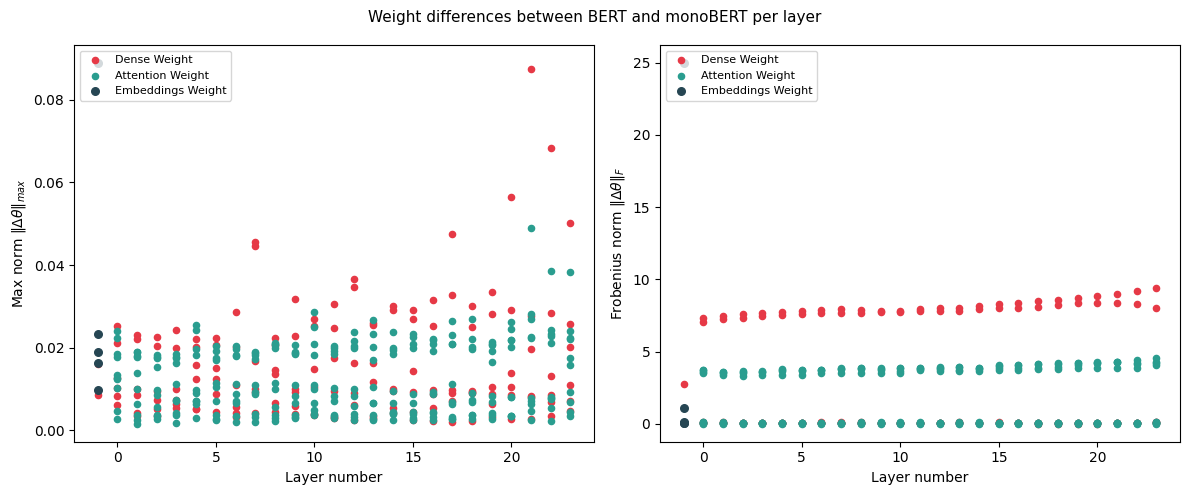
\includegraphics[width=0.92\textwidth]{figures/matrix_change_analysis.png}
    \caption{Matrix-level parameter differences between BERT and MonoBERT. Frobenius norm measures the overall magnitude of change, while max norm measures the largest individual weight difference. The observed changes motivate the selected attention-matrix adaptation experiments.}
    \label{fig:matrix_change_analysis}
\end{figure}

\FloatBarrier

Figure~\ref{fig:embedding_distance_analysis} reports embedding-level differences between BERT and MonoBERT using Euclidean distance and cosine similarity. The analysis was used to select the six embedding rows with the largest observed changes for the top-6 embedding experiment.

\begin{figure}[H]
    \centering
    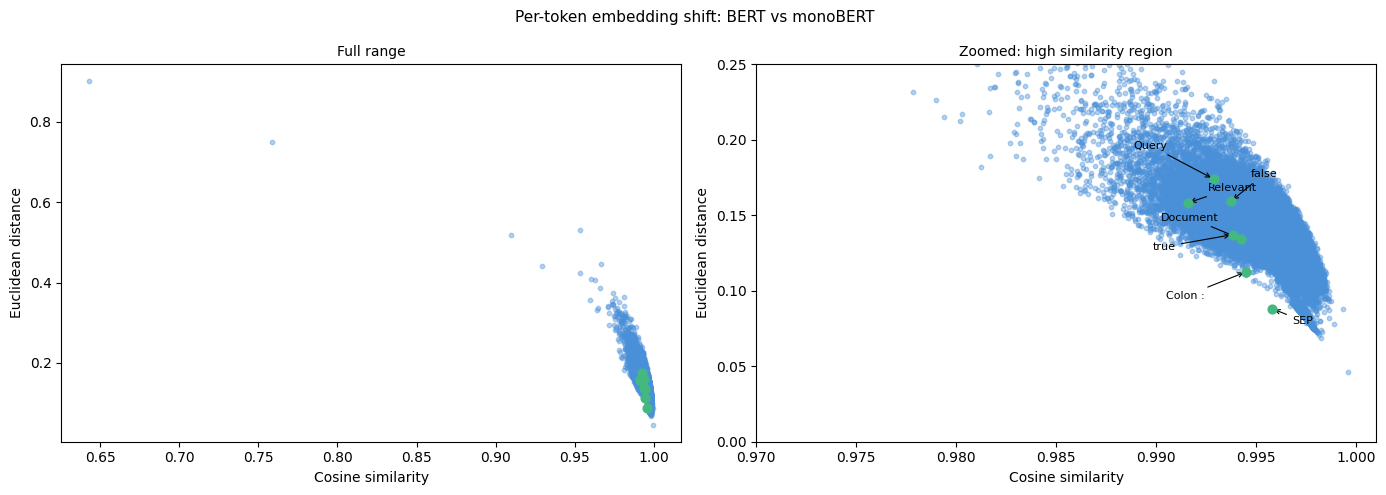
\includegraphics[width=0.92\textwidth]{figures/embedding_distance_analysis.png}
    \caption{Embedding-level differences between BERT and MonoBERT. Each point represents a vocabulary embedding vector. Euclidean distance measures magnitude of change, while cosine similarity measures directional change. The analysis motivates the selected embedding experiments.}
    \label{fig:embedding_distance_analysis}
\end{figure}

\FloatBarrier

\section{Overall Results}
\label{sec:results_overview}

The evaluation covers ten approaches across four datasets: TREC DL 2019, TREC DL 2020, MS MARCO dev small, and DL-Hard. The main metric discussed is nDCG@10 because it measures ranking quality at the top of the result list, which is the most important part of the ranking in a re-ranking setting. MRR@10, MAP@1000, and Recall@100 are also reported.

\begin{table}[ht]
\centering
\small
\begin{tabular}{lrcccc}
\hline
\textbf{Approach} & \textbf{Params} & \textbf{DL19} & \textbf{DL20} & \textbf{Dev Small} & \textbf{DL-Hard} \\
\hline
BM25 & 0 & 0.4138 & 0.4475 & 0.2302 & 0.2513 \\
CLS/SEP embeddings & 2,048 & 0.0449 & 0.0224 & 0.0093 & 0.0031 \\
Top-6 embeddings & 6,144 & 0.0197 & 0.0193 & 0.0054 & 0.0016 \\
LoRA top-3 attention & 49,152 & 0.5266 & 0.4825 & 0.2955 & 0.2873 \\
LoRA all attention & 1,572,864 & \textbf{0.6595} & 0.6762 & 0.4207 & \textbf{0.4006} \\
Top-3 attention matrices & 3,145,728 & 0.5627 & 0.5312 & 0.3348 & 0.3065 \\
All embeddings except CLS/SEP & 31,252,480 & 0.0274 & 0.0123 & 0.0066 & 0.0006 \\
All embeddings & 31,254,528 & 0.0510 & 0.0450 & 0.0173 & 0.0151 \\
Full MonoBERT & 335,143,938 & 0.6286 & 0.6426 & 0.4059 & 0.3977 \\
Public MonoBERT & --\textsuperscript{*} & 0.6540 & 0.6856 & 0.4297 & 0.3965 \\
\hline
\end{tabular}
\caption{nDCG@10 results across all evaluated approaches and datasets, ordered by number of trained parameters, from BM25 (no neural parameters) to full fine-tuning. The BM25 baseline is recomputed directly with PyTerrier over the MS MARCO passage index. \textsuperscript{*}Public MonoBERT is an externally released checkpoint and was not trained locally.}
\label{tab:results_nDCG}
\end{table}

\begin{table}[ht]
\centering
\small
\begin{tabular}{lrcccc}
\hline
\textbf{Approach} & \textbf{Params} & \textbf{DL19} & \textbf{DL20} & \textbf{Dev Small} & \textbf{DL-Hard} \\
\hline
BM25 & 0 & 0.4422 & 0.5056 & 0.6772 & 0.4007 \\
CLS/SEP embeddings & 2,048 & 0.1379 & 0.1202 & 0.1735 & 0.0475 \\
Top-6 embeddings & 6,144 & 0.0462 & 0.0306 & 0.0356 & 0.0112 \\
LoRA top-3 attention & 49,152 & 0.4669 & 0.5254 & 0.7433 & 0.4708 \\
LoRA all attention & 1,572,864 & \textbf{0.5229} & 0.5552 & 0.7890 & 0.5059 \\
Top-3 attention matrices & 3,145,728 & 0.4707 & 0.5331 & 0.7635 & 0.4741 \\
All embeddings except CLS/SEP & 31,252,480 & 0.1370 & 0.1655 & 0.2057 & 0.1244 \\
All embeddings & 31,254,528 & 0.3230 & 0.3291 & 0.5566 & 0.3321 \\
Full MonoBERT & 335,143,938 & 0.4706 & 0.5310 & 0.7809 & 0.4863 \\
Public MonoBERT & --\textsuperscript{*} & 0.5224 & \textbf{0.5680} & \textbf{0.7929} & \textbf{0.5217} \\
\hline
\end{tabular}
\caption{Recall@100 results across all evaluated approaches and datasets, ordered by number of trained parameters, from BM25 (no neural parameters) to full fine-tuning. \textsuperscript{*}Public MonoBERT is an externally released checkpoint and was not trained locally.}
\label{tab:results_recall}
\end{table}

\begin{table}[ht]
\centering
\small
\begin{tabular}{llcccc}
\hline
\textbf{Approach} & \textbf{Metric} & \textbf{DL19} & \textbf{DL20} & \textbf{Dev Small} & \textbf{DL-Hard} \\
\hline
Public MonoBERT & MRR@10 & \textbf{0.9814} & 0.9250 & \textbf{0.3706} & 0.6335 \\
LoRA all attention & MRR@10 & 0.9709 & \textbf{0.9414} & 0.3619 & 0.6712 \\
Full MonoBERT & MRR@10 & 0.9690 & 0.9290 & 0.3453 & \textbf{0.6815} \\
\hline
Public MonoBERT & MAP@1000 & \textbf{0.4722} & \textbf{0.4718} & \textbf{0.3730} & 0.2676 \\
LoRA all attention & MAP@1000 & 0.4697 & 0.4686 & 0.3651 & \textbf{0.2761} \\
Full MonoBERT & MAP@1000 & 0.4248 & 0.4285 & 0.3488 & 0.2585 \\
\hline
\end{tabular}
\caption{MRR@10 and MAP@1000 for the strongest neural re-rankers.}
\label{tab:results_mrr_map_best}
\end{table}

The results show a clear separation between embedding-only adaptation methods and methods that modify transformer attention or perform broader model adaptation. The strongest-performing approaches are Public MonoBERT, Full MonoBERT, and LoRA applied to all attention matrices. In contrast, all embedding-only methods perform substantially worse, even when the full embedding layer is trained.

\section{BM25 and MonoBERT Baselines}
\label{sec:results_baselines}

BM25 serves as the lexical baseline. Its performance is substantially lower than the neural re-ranking models across all datasets, achieving nDCG@10 scores of 0.4138 on TREC DL 2019, 0.4475 on TREC DL 2020, 0.2302 on MS MARCO dev small, and 0.2513 on DL-Hard. Although its absolute performance on DL-Hard remains modest, BM25 performs relatively better than several embedding-based approaches. This is likely because the DL-Hard candidate set was originally generated using BM25, making the evaluation pool inherently aligned with its retrieval strategy.

Public MonoBERT substantially outperforms BM25 on every dataset, which shows the effectiveness of neural cross-encoder re-ranking. The improvements are particularly pronounced on TREC DL 2019 and TREC DL 2020, where it achieves nDCG@10 scores of 0.6540 and 0.6856, respectively. These results highlight the advantage of full query-passage interaction within the BERT architecture.

Full MonoBERT is included to verify that the locally trained implementation produces results comparable to the publicly released model. Across all datasets, its performance closely matches that of Public MonoBERT, although the public model consistently achieves slightly higher scores. Full MonoBERT attains nDCG@10 values of 0.6286 on TREC DL 2019, 0.6426 on TREC DL 2020, 0.4059 on MS MARCO dev small, and 0.3977 on DL-Hard. The similarity between the two models indicates that the local training and evaluation pipeline is functioning as expected.

\section{Embedding-Level Adaptation}
\label{sec:results_embedding}

The main proposed approach trains only the embeddings of \texttt{[CLS]} and \texttt{[SEP]}. This updates only 2048 parameters, making it the smallest neural adaptation method in the thesis. However, the ranking performance is weak. It obtains nDCG@10 values of 0.0449 on TREC DL 2019, 0.0224 on TREC DL 2020, 0.0093 on MS MARCO dev small, and 0.0031 on DL-Hard.

These results show that the special-token embeddings alone are not sufficient to adapt BERT-large into an effective passage re-ranker. The result is important because it directly addresses the main transfer question from Light-MonoT5 to MonoBERT. Although \texttt{[CLS]} and \texttt{[SEP]} are structurally important in BERT, updating their embeddings does not provide enough control over the internal query-passage interaction behavior of the model.

The top-6 embedding experiment performs even weaker in most cases. This experiment was motivated by the embedding distance analysis between BERT and MonoBERT. However, during training, only four of the six selected embedding rows changed. The remaining selected tokens did not appear in the tokenized training inputs and therefore did not receive gradient updates. This reveals a practical limitation of selected embedding tuning: selecting an embedding row is not sufficient if the corresponding token is rare or absent during training.

The all-embedding experiment provides a more informative comparison. It trains the entire embedding matrix while freezing the rest of the model. This approach improves Recall@100 substantially in some cases, especially on MS MARCO dev small where it reaches 0.5566. However, its nDCG@10 remains low. This suggests that embedding adaptation can move some relevant passages higher in the ranking, but it does not learn the fine-grained ordering needed for strong top-10 performance.

The all-embeddings-except-\texttt{[CLS]}/\texttt{[SEP]} experiment also performs poorly. This indicates that ordinary vocabulary embeddings alone are not sufficient to adapt the frozen model. It also provides an indirect contrast with the \texttt{[CLS]}/\texttt{[SEP]} experiment: the structural tokens appear to contribute more than ordinary vocabulary embeddings, but neither structural-token tuning nor non-structural embedding tuning is sufficient on its own.

Overall, the embedding-level experiments show that embeddings are too limited as the sole adaptation mechanism for MonoBERT-style re-ranking. They influence the initial token representations, but they do not directly modify the internal transformer computations responsible for modeling query-passage interactions.

\section{Attention-Based Adaptation}
\label{sec:results_attention}

The attention-based methods perform substantially better than the embedding-only methods. The top-3 attention matrix experiment trains the three matrices that changed most in the BERT-to-MonoBERT analysis. It achieves nDCG@10 values of 0.5627 on TREC DL 2019 and 0.5312 on TREC DL 2020, while also performing strongly on MS MARCO dev small and DL-Hard.

This result provides evidence that the parameter-change analysis successfully identified attention matrices that are important for retrieval adaptation. The selected matrices were not chosen randomly; rather, they were selected because they exhibited the largest changes between BERT and MonoBERT. Their strong performance supports the hypothesis that the analysis identified parts of the model that play an important role in IR adaptation.

The results also support a broader interpretation that passage re-ranking relies heavily on attention-level interactions. Since cross-encoders allow query and passage tokens to interact through self-attention, modifying attention matrices directly affects one of the primary mechanisms responsible for relevance matching. This likely explains why attention-matrix tuning performs substantially better than embedding-only tuning.

An interesting comparison is between direct tuning of the selected attention matrices and applying LoRA to the same matrices. Direct optimization consistently achieves higher effectiveness than LoRA top-3 attention, reaching nDCG@10 scores of 0.5627 versus 0.5266 on TREC DL 2019 and 0.5312 versus 0.4825 on TREC DL 2020. This suggests that, for a very small subset of attention modules, directly updating the original parameters is more effective than constraining the updates to low-rank adapters, although LoRA remains considerably more parameter-efficient.

\section{LoRA Results}
\label{sec:results_lora}

LoRA applied to all attention matrices is the strongest parameter-efficient method evaluated in this thesis. It performs comparably to both Public MonoBERT and Full MonoBERT across all datasets. On TREC DL 2019, it achieves an nDCG@10 of 0.6595, slightly exceeding both Public MonoBERT (0.6540) and Full MonoBERT (0.6286). On TREC DL 2020, it reaches 0.6762, remaining close to Public MonoBERT's 0.6856.

These results show that LoRA is a strong PEFT baseline for passage re-ranking. By adapting the attention computations without updating the full set of model parameters, it preserves most of the effectiveness of full fine-tuning while requiring substantially fewer trainable parameters.

LoRA top-3 attention performs worse than LoRA all attention, but remains competitive relative to its parameter count. It achieves nDCG@10 scores of 0.5266 on TREC DL 2019 and 0.4825 on TREC DL 2020, while also maintaining strong Recall@100 values across the evaluated datasets. This indicates that applying LoRA only to the most important attention matrices can retain a substantial portion of the performance achieved by broader LoRA adaptation.

The comparison between LoRA all attention and LoRA top-3 attention is particularly relevant to the thesis. It suggests that parameter-change analysis can guide not only direct parameter tuning, but also the placement of parameter-efficient adaptation modules. Rather than applying LoRA uniformly across all attention layers, the results indicate that concentrating adaptation on a small number of carefully selected modules remains an effective strategy.

\section{Efficiency and Parameter Trade-offs}
\label{sec:results_efficiency}

The experiments show that the number of trainable parameters alone does not determine ranking performance. The \texttt{[CLS]}/\texttt{[SEP]} experiment is extremely parameter-efficient, yet its ranking effectiveness is poor. Conversely, the all-embedding experiment trains substantially more parameters than the \texttt{[CLS]}/\texttt{[SEP]} approach but still performs considerably worse than the attention-based methods.

These results suggest that the location of adaptation is more important than the number of trainable parameters alone. Parameters within the attention layers have a much greater influence on ranking effectiveness because they largely determine how query and passage tokens interact throughout the transformer. In contrast, embedding parameters affect only the initial token representations before they are processed by the frozen transformer layers.

The top-3 attention and LoRA top-3 attention experiments provide a useful compromise between parameter efficiency and ranking effectiveness. Although they update only a small fraction of the model compared with full fine-tuning or LoRA all attention, they substantially outperform all embedding-only approaches. This indicates that carefully selected attention modules constitute effective adaptation targets for BERT-based passage re-ranking.

\begin{table}[ht]
\centering
\small
\resizebox{\textwidth}{!}{%
\begin{tabular}{l r p{6.5cm}}
\hline
\textbf{Approach} & \textbf{Updated Parameters} & \textbf{Main Updated Component} \\
\hline
BM25 & 0 & No neural parameters \\
Public MonoBERT & -- & Public fully fine-tuned model \\
CLS/SEP embeddings & 2,048 & Two special-token embeddings \\
Top-6 embeddings & 6,144 & Six selected embedding rows \\
Top-3 attention matrices & 3,145,728 & Three full attention matrices \\
All embeddings & 31,254,528 & Full word embedding matrix \\
All embeddings except CLS/SEP & 31,252,480 & Word embeddings except token IDs 101 and 102 \\
LoRA all attention & 1,572,864 & Low-rank adapters in all attention matrices \\
LoRA top-3 attention & 49,152 & Low-rank adapters in selected attention matrices \\
Full MonoBERT & 335,143,938 & All model parameters \\
\hline
\end{tabular}%
}
\caption{Number of updated parameters for each approach. The table highlights the efficiency-effectiveness trade-off between highly restricted embedding-level methods, attention-level methods, LoRA variants, and full fine-tuning.}
\label{tab:updated_parameters}
\end{table}

\section{Discussion}
\label{sec:results_interpretation}

The results clarify the relationship between Light-MonoT5 and MonoBERT. The Light-MonoT5 idea motivates the hypothesis that selected embeddings may control task-specific behavior. In the BERT setting, this hypothesis is only partially supported. Special-token embeddings can be trained successfully, and the gradient masking works as intended, but the resulting ranking model is not competitive with attention-based adaptation methods.

One possible explanation is the architectural difference between MonoT5 and MonoBERT. MonoT5 and MonoBERT use different mechanisms for relevance prediction. MonoT5 is a sequence-to-sequence model where prompt tokens can directly influence the generated output. In contrast, MonoBERT predicts relevance from the final \texttt{[CLS]} representation after multiple layers of self-attention. Therefore, changing only the initial \texttt{[CLS]} and \texttt{[SEP]} embeddings may not provide sufficient control over the final relevance prediction process.

The strongest evidence from the experiments is that attention-layer adaptation is substantially more effective than embedding-layer adaptation for BERT-based passage re-ranking. Attention matrices influence how query and passage tokens interact throughout the transformer layers. Since relevance depends on modelling relationships between the query and passage, modifying attention components appears to provide a more effective adaptation mechanism than modifying only the input embeddings.

\section{Answers to Research Questions}
\label{sec:results_rq}

\justifying

\begin{description}

\item[\textbf{RQ1}] \textbf{Can a BERT cross-encoder be adapted by training only selected embeddings?}

\vspace{-0.4\baselineskip}

Selected embeddings can be trained successfully, but the resulting ranking performance is weak. Therefore, embedding-only tuning is possible, but it is not competitive with attention-based adaptation methods.

\vspace{0.6\baselineskip}

\item[\textbf{RQ2}] \textbf{How does CLS/SEP tuning compare with top-changed embedding tuning?}

\vspace{-0.4\baselineskip}

The \texttt{[CLS]}/\texttt{[SEP]} method generally performs better than the top-6 embedding method, although both approaches remain substantially weaker than attention-based methods. The top-6 method is additionally limited by the fact that some selected embedding rows did not appear during training and therefore did not receive updates.

\vspace{0.6\baselineskip}

\item[\textbf{RQ3}] \textbf{Are useful changes concentrated more in embeddings or attention matrices?}

\vspace{-0.4\baselineskip}

The results indicate that attention matrices are substantially more effective adaptation targets than embeddings for BERT-based passage re-ranking.

\vspace{0.6\baselineskip}

\item[\textbf{RQ4}] \textbf{How does embedding-level tuning compare with LoRA?}

\vspace{-0.4\baselineskip}

LoRA is substantially stronger than embedding-level tuning. LoRA applied to all attention matrices performs close to MonoBERT, while embedding-only methods remain far below this level of effectiveness.

\vspace{0.6\baselineskip}

\item[\textbf{RQ5}] \textbf{Can LoRA on the top-3 changed matrices retain much of LoRA all attention performance?}

\vspace{-0.4\baselineskip}

Yes. LoRA top-3 attention performs worse than LoRA all attention, but it retains a substantial portion of the ranking effectiveness while requiring significantly fewer trainable parameters.

\vspace{0.6\baselineskip}

\item[\textbf{RQ6}] \textbf{Does Full MonoBERT validate the setup?}

\vspace{-0.4\baselineskip}

Yes. Full MonoBERT performs close to Public MonoBERT, indicating that the local training and evaluation pipeline is broadly aligned with MonoBERT-style passage re-ranking.

\end{description}


\section{Summary}
\label{sec:results_summary}

The main conclusion from the results is that embedding-level tuning is informative but not sufficient for strong BERT-based passage re-ranking. The most effective adaptation mechanisms evaluated in this thesis are attention-based. LoRA applied to all attention matrices performs close to MonoBERT, while LoRA top-3 attention and direct top-3 attention matrix tuning provide effective restricted alternatives with fewer trainable parameters.

Overall, the experiments suggest that adaptation location is more important than parameter count alone. Although embedding-level methods modify the input representation space, attention-level methods provide a more direct mechanism for modifying query-passage interaction behaviour, which is central to cross-encoder passage re-ranking.
\chapter{Conclusions}
\label{ch:conclusions}

This thesis investigated highly parameter-efficient adaptation strategies for BERT-based passage re-ranking, with a particular focus on embedding-level tuning as an alternative to LoRA-based adaptation. The work began from the motivation of Light-MonoT5, where selected prompt-token embeddings are trained while the rest of the model remains frozen. The central question was whether a similar idea could be transferred to a MonoBERT-style cross-encoder.

\section{Summary of the Thesis}
\label{sec:conclusions_summary}

The thesis studied passage re-ranking using \texttt{bert-large-uncased}. The main proposed approach trained only the embeddings of the BERT structural tokens \texttt{[CLS]} and \texttt{[SEP]}. These tokens are central to the MonoBERT input format:

\begin{equation}
    \texttt{[CLS]} \; q \; \texttt{[SEP]} \; d \; \texttt{[SEP]}.
\end{equation}

The motivation was that these structural tokens occur in every query-passage pair and may influence how the frozen model organizes the input. Training only these two embeddings updates just 2048 parameters, making it an extremely small adaptation method.

To better understand where task adaptation occurs, the thesis also compared BERT and MonoBERT parameters. The most changed embedding rows and attention matrices were selected for additional experiments. The final experimental setup included ten approaches: BM25, Public MonoBERT, \texttt{[CLS]}/\texttt{[SEP]} tuning, top-6 embedding tuning, top-3 attention matrix tuning, all-embedding tuning, all embeddings except \texttt{[CLS]}/\texttt{[SEP]}, LoRA all attention, LoRA top-3 attention, and Full MonoBERT.

The methods were evaluated on TREC DL 2019, TREC DL 2020, MS MARCO dev small, and DL-Hard. The results revealed a consistent pattern. Embedding-only adaptation was highly parameter-efficient but weak in ranking effectiveness. Methods that modified attention components or performed broader model adaptation were substantially stronger. LoRA applied to all attention matrices performed close to Public MonoBERT and Full MonoBERT, while LoRA applied only to the top-3 changed attention matrices retained a large portion of the performance with far fewer trainable parameters.

\section{Main Findings}
\label{sec:conclusions_findings}

The first finding is that training only \texttt{[CLS]} and \texttt{[SEP]} is not sufficient for strong passage re-ranking. Although the method is extremely efficient, its ranking performance is far below MonoBERT and LoRA. This shows that updating only the BERT structural tokens does not provide enough adaptation capacity for strong passage re-ranking.

The second finding is that training more embeddings does not automatically solve the problem. The full embedding-layer experiment improves recall in some cases, but it still performs poorly in terms of top-ranking quality. The all-embeddings-except-\texttt{[CLS]}/\texttt{[SEP]} experiment also remains weak. These results suggest that embedding-level adaptation alone does not sufficiently modify the internal query-passage interaction mechanisms required for strong re-ranking.

The third finding is that attention matrices are substantially more effective adaptation targets than embeddings in this experimental setting. Directly training the top-3 changed attention matrices produces strong results. This provides further evidence that the BERT-to-MonoBERT parameter-change analysis identifies meaningful parts of the model for retrieval adaptation.

The fourth finding is that LoRA is a strong PEFT baseline for this task. LoRA applied to all attention matrices performs close to the performance of fully fine-tuned MonoBERT models while training far fewer parameters than full fine-tuning. LoRA applied only to the top-3 changed attention matrices is weaker, but still much stronger than embedding-only adaptation.

\section{Limitations}
\label{sec:conclusions_limitations}

The thesis has several limitations. First, the experiments focus on BERT-based passage re-ranking and do not evaluate embedding-level tuning across many different language model architectures. The original thesis proposal included the broader possibility of evaluating generalization across models and tasks, but the final experimental work focuses on BERT and MonoBERT because of time and computational constraints.

Second, the maximum input length is set to 128 tokens for computational feasibility. This makes the experiments manageable, but it may truncate useful passage content. A longer maximum sequence length could potentially improve ranking performance, especially for full MonoBERT and LoRA models.

Third, the evaluation focuses on MS MARCO, TREC DL, and DL-Hard. BEIR is discussed as an important benchmark, but broad out-of-domain BEIR evaluation was not completed in the final experimental set. Evaluating on more BEIR datasets would provide a stronger test of generalization.

Fourth, the parameter-change analysis depends on the specific BERT and MonoBERT models compared. Different checkpoints or training settings might produce different top-changed embeddings and matrices.

\section{Future Work}
\label{sec:conclusions_future}

Future work could explore hybrid adaptation strategies. The results suggest that embeddings alone are not sufficient, but they may still be useful when combined with selected attention modules. For example, one could train \texttt{[CLS]} and \texttt{[SEP]} together with LoRA adapters on selected attention matrices.

Another direction is to evaluate the approach on more datasets, especially from BEIR. This would test whether the conclusions hold beyond MS MARCO-style passage ranking. It would also allow the thesis question to be extended toward out-of-domain generalization.

A third direction is to apply the same methodology to other architectures. The architectural difference between MonoT5 and MonoBERT may explain why prompt-token adaptation transfers differently between the two settings. Testing the same parameter-selection idea on T5, BERT, and newer decoder-only re-rankers would clarify whether embedding-level PEFT is architecture-dependent.

Finally, future work could investigate more advanced parameter-selection criteria. This thesis uses norm-based differences between BERT and MonoBERT. Other criteria could include gradient magnitude, Fisher information, activation sensitivity, or task-vector composition.

\section{Final Remarks}
\label{sec:conclusions_final}

The thesis shows that embedding-level tuning is a useful tool for studying adaptation behaviour, but it does not achieve competitive ranking effectiveness compared with LoRA-based adaptation in BERT-based passage re-ranking. The results indicate that effective adaptation for MonoBERT appears to depend more strongly on attention mechanisms than on isolated embedding vectors. Therefore, the most promising direction for efficient BERT re-ranking is not purely embedding-level adaptation, but targeted attention-level adaptation guided by parameter-change analysis.
%-------------------------------------------------------------------------------
% \backmatter
%-------------------------------------------------------------------------------
% Uncomment if you use acronyms

%\phantomsection
%\pdfbookmark[1]{List of Acronyms}{listofacronyms}
%\printglossary[type=\acronymtype]
%-------------------------------------------------------------------------------
\include{backmatter}
%-------------------------------------------------------------------------------
\end{document}
%-------------------------------------------------------------------------------